%% LaTeX2e class for student theses
%% sections/content.tex
%% 
%% Karlsruhe Institute of Technology
%% Institute for Program Structures and Data Organization
%% Chair for Software Design and Quality (SDQ)
%%
%% Dr.-Ing. Erik Burger
%% burger@kit.edu
%% burger@kit.edu
%%
%% Version 1.3.3, 2018-04-17

\chapter{Grundlagen}
\label{ch:Grundlagen}

\section{Nachrichtenbasierte Middleware (MOM)}
Ereignissbasierte Systeme bestehen aus Ereignissen, Sendern, Empfängern und einer Middleware \cite{Carzaniga1998}. In einem solchen System werden Ereignisse von einem Sender instanziiert und von einem Empfänger entgegengenommen. Ereignisse sind dabei signifikante Änderungen eines Zustands (chandy06). Unter signifikant versteht man Änderungen, die das System beeinflussen. Dieser Transport von Ereignissen zwischen Sender und Empfänger wird durch die Middleware ermöglicht. Eine solche Middleware nennt man eine nachrichtenbasierte Middleware (MOM) \cite{Curry05}. Diese bietet eine Infrastruktur zum asynchronen Senden und Empfangen von Nachrichten, in verteilten Systemen an. Teilnehmer einer MOM müssen nicht blockieren und warten, wenn sie eine Nachricht gesendet haben oder empfangen wollen. Dieser asynchroner Mechanismus ist ein großer Vorteil. Außerdem führen MOMs eine Vermittlerschicht zwischen Sender und Empfänger ein, die für den Nachrichtenaustausch genutzt wird. Diese Zwischenschicht führt zu einer losen Kopplung der einzelnen Komponenten.  \\
%- Vorteile \\
%- Standards \\
%-- wie jms and amqp \\

\subsection{Architektur}
MOMs unterscheiden sich, neben ihrer Implementierung, in ihrer Architektur. Es gibt drei verschiedene Architekturen für MOMs.
\begin{itemize}
\item Die \textbf{Peer-To-Peer} Architektur, hat keinen ausgewählten Knoten, der die MOM bereitstellt. Die Funktionalität, die zum kommunizieren benötigt wird, wird von den Sendern und Empfängern bereitgestellt.
\item In der \textbf{zentralen} Variante läuft die MOM auf einem Zentralen Knoten. Alle Sender und Empfänger sind mit diesem Knoten verbunden. 
\item Schließlich gibt es noch die \textbf{verteilte} Architektur. Die MOM ist über mehrere Knoten verteilt. Der Austausch von Daten wird mithilfe von Routing-Algorithmen bewerkstelligen. Sender und Empfänger müssen nicht mit dem selben Middlewareknoten verbunden sein.
\end{itemize}  

\subsection{Warteschlangen}
Warteschlangen sind ein wichtiger Bestandteil von MOMs, vor allem für deren asynchronen Nachrichtenaustausch. Sender nutzen sie um Nachrichten hinzuschicken. Empfänger nutzen sie um Nachrichten abzuholen. Die Nachrichten in der Warteschlange sind nach einer festgelegten Ordnung geordnet, z.B. First-In-First-Out, also die Nachricht, die als erstes in die Warteschlange eingefügt wurde, wird auch als erste wieder herausgenommen. Eine Warteschlange kann i.d.R. von einem Nutzer konfiguriert werden. Mögliche Konfigurationen für eine Warteschlange können Größe, Verweildauer oder Sortierung sein.

\subsection{Nachrichtenmodelle}
\label{sec:nachrichtenmodelle}
Wie eine MOM Nachrichten austauscht, wird in ihrem Nachrichtenmodell festgelegt. Man unterscheidet dabei zwischen dem Point-To-Point und dem Publish/Subscribe Modell. Eine MOM kann auch aus einer Kombination der beiden Modelle bestehen um auf bestimmte Szenarien reagieren zu können.
\begin{itemize}
\item Im \textbf{Point-To-Point} Modell werden Nachrichten von einem Sender an eine bestimmte  Warteschlange gesendet. Normalerweise ist eine Warteschlange mit genau einem Empfänger verbunden. Es können aber auch mehrere Empfänger mit einer Warteschlange verbunden sein. Die Nachrichten werden in diesem Fall nach dem First-Come-First-Serve (FCFS) Prinzip entnommen und verarbeitet. 
\item Beim \textbf{Publish/Subscriber} Modell verbindet sich der Empfänger (Subscriber) mit der MOM und legt, für die Nachrichten die er Empfangen möchte, Bedingungen fest (Eugster 03). Dabei wird zwischen drei Arten von Bedingungen unterschieden \cite{Rathfelder2013}:
\begin{itemize}
    \item Inhaltsbasiert: Dabei lassen sich Filterregeln definieren, die auf den Inhalt und die Payload der Nachrichten angewendet werden können.
    \item Kanalbasiert: Die MOM bietet verschiedene Kanäle (Channel) an, an die Nachrichten gesendet werden können. Empfänger können sich an einem Kanal anmelden und erhalten alle Nachrichten, die an diesen Kanal gesendet werden.
    \item Typbasiert: Die Nachrichten werden anhand ihres Typs identifiziert und an die Empfänger weitergeleitet.
\end{itemize}
\end{itemize}

\subsection{Interaktionstypen}
?
\begin{itemize}
    \item 1:1
    \item 1:n
    \item m:1
    \item m:n
\end{itemize}
\subsection{Grad der Entkopplung}
?
\begin{itemize}
    \item Synchronisation
    \item Raum
    \item Zeit
\end{itemize}
\section{Java Message Service (JMS)}
Der Java Message Service (JMS) ist eine standardisierte Programmierschnittstelle (API) (Hapner JMS Specification). Sie dient dazu Java Applikationen Zugriff auf nachrichtenbasierten Middlewares zu geben. Im JMS Umfeld wird die MOM als JMS Server und die Applikationen die die API verwenden, um Nachrichten auszutauschen, als JMS Klienten bezeichnet. JMS ist Teil der Java Platform Enterprise Edition, die Standards für Enterprise Applikationen definiert. JMS unterstützt verschiedene Nachrichtentypen, wie Text-, Byte- oder Objektnachrichten. Es werden die beiden oben vorgestellten Nachrichtenmodelle, Punkt-Zu-Punkt und Publish/Subscriber Modell unterstützt.
Die API wird bei der Untersuchung der MOM und bei der Evaluierung benötigt.

\section{Modellgetriebene Softwareentwicklung}
In der modellgetriebenen Software-Entwicklung \cite{MDSD} werden Teile des Software-Systems innerhalb von Modellen unter Nutzung von Abstraktionen beschrieben. Modelle sind Entwicklungsartefakte und Systembestandteile oder erlauben das automatische Ableiten von Systemartefakten. Das Ziel der modellgetriebenen Softwareentwicklung ist, die Verbesserung der Softwarequalität und der Wiederverwendbarkeit. Außerdem soll eine Erhöhung der Entwicklungseffizienz, zum Beispiel durch Quellcodeerzeugung, aus den Modellen erreicht werden.

\subsection{Modell}
Nach Herbert Stachowiak \cite{Stachowiak1973} zeichnet sich ein Modell durch die folgenden drei Merkmale aus.
\begin{itemize}
\item \textbf{Abbildung} - Bei einem Modell handelt es sich um eine Abbildung oder Repräsentation von einem künstlichen oder natürlichen Original. Das Original kann selbst wieder ein Modell sein. 
\item \textbf{Verkürzung} - Es werden nicht alle Attribute des Originals erfasst, sondern nur diejenigen, die relevant sind.
\item \textbf{Pragmatismus} - Modelle erfüllen ihre Ersatzfunktion für bestimmte Subjekte, innerhalb einer bestimmten Zeit und unter Einschränkung bestimmter gedanklicher oder tätlicher Operationen. Beispielsweise benötigt eine Analyse je nach gewünschter Genauigkeit, unterschiedlich genaue Modelle. Der Pragmatismus schreibt vor, dass man hier nicht unnötig genau arbeitet.
\end{itemize} 
\subsection{Meta-Modell}
Ein Meta-Modell beschreibt die Struktur eines Modells. Dabei muss ein Meta-Modell die folgenden Bereiche abdecken:
\begin{itemize}
\item \textbf{Abstrakte Syntax}: Sie beschreibt die Konstrukte, aus denen die Modelle bestehen, sowie deren Eigenschaften und Beziehungen.
\item \textbf{Konkrete Syntax}: Diese beschreibt die Darstellung der Konstrukte, Eigenschaften und Beziehungen, die in der abstrakten Syntax spezifiziert sind.
\item \textbf{Statische Semantik}: Mithilfe dieser werden Modellierungsregeln und Einschränkungen ausgedrückt, die mit der abstrakten Syntax nicht möglich sind.
\item \textbf{Dynamische Semantik}: Sie drückt die Bedeutung der Konstrukte aus und wird oft nicht formal, sondern durch natürlich sprachlichen Text spezifiziert.
\end{itemize}

\subsection{Modeltransformation}
Bei der Modelltransformation (Kleppe, Warmer und Bast 2003) wird ein Quellmodell in ein Zielmodell übersetzt. Dies geschieht mithilfe einer Transformationsdefinition. Die Transformationsdefinition besteht aus einer Menge von Transformationsregeln, die beschreiben wie ein Modell in ein anderes überführt wird. Dabei wird zwischen zwei Arten der Modelltransformation unterschieden:
\begin{itemize}
    \item Modell-Zu-Modell: Dabei wird ein Quellmodell, dass zu einem Quellmetamodell konform ist in ein Zielmodell, dass zu einem Zielmetamodell konform ist, transformiert.
    \item Modell-Zu-Text: Dabei wird ein Modell in eine oder mehrere Textdateien übersetzt. Meistens beinhalten diese Quellcode einer gegebenen Programmiersprache. Eine Transformation kann aber auch Dokumentation oder Konfiguartionen generieren.
\end{itemize}
Für die Masterarbeit wurde eine Modell-Zu-Modell Transformation beschrieben/entwickelt.
\section{Palladio Komponenten Modell}
\label{sec:palladio}
Das Palladio Komponentenmodell (PCM) \cite{palladio17} ist eine Architecture-Description-Language (ADL) und unterstützt die Erstellung skalierbarer, zuverlässiger, wartbarer und wiederverwendbarer komponenentenbasierter Softwarearchitekturen. Neben der Beschreibung sind auch Qualitätsanalysen, wie etwa bezüglich der Performanz oder Zuverlässigkeit möglich. Im Folgenden werden Teile des PCM erklärt, die für die Masterarbeit benötigt werden.

%\subsection{Viewpoints}
%- structural (assembly) \\
%- behaviour (sequence?) \\
%- deployment (allocation, deployment decision) \\
\subsection{Rollen}
%s.203
Die Modellierung der verschiedenen MOMs erfolgt mithilfe von Software-Architektur-Modellen. In der modellgetriebenen Softwareentwicklung und in Palladio gibt es dabei verschiedene Rollen, die an unterschiedlichen Teilen der Architektur arbeiten und dort ihr spezifisches Wissen einbringen.
\begin{itemize}
\item Die Architektur und der Zusammenhang der einzelnen Komponenten
miteinander werden vom \textbf{Softwarearchitekt} entworfen. Er ist auch dafür
zuständig weitere Anweisungen an die anderen Rollen weiterzugeben. Gleichzeitig ist er für das \textbf{System-Modell} zuständig, das die Zusammensetzung der Komponenten charakterisiert.
\item Das Wissen darüber, wie der Benutzer mit dem System interagiert
und welche Parameter im Kontrollfluss verwendet werden, stammt vom \textbf{Domänenxperten}. Die Modellierung wird im \textbf{Usage-Modell} festgehalten.
\item Für das Implementieren und Spezifizieren der einzelnen
Komponenten ist der \textbf{Komponentenentwickler} verantwortlich. Diese modelliert er im \textbf{Komponen-ten-Repository-Modell}. Es enthält die einzelnen Komponenten und Schnittstellen.
\item Die Zusammenstellung der Systemumgebung der Software wird vom \textbf{Softwareverteilungsexperten} übernommen. Diese wird von ihm im \textbf{Ausführungsum-gebungs-Modell} festgehalten. Außerdem weist der Softwareverteilungsexperte den Komponenten Ressourcen zu. Dies hält er im \textbf{Komponenten-Allokations-Modell} fest.
\end{itemize}
Die Modelle, die von den verschiedenen Rollen entwickelt und gewartet werden, bilden zusammen eine Palladio Modell Instanz. Mithilfe der Modellierung einer MOM sollen die verschiedenen Rollen unterstützt werden. 
\subsection{Qualitätsattribute}
\subsubsection{Performanz} 
%(Buch S. 93/94)
Performanz ist bezüglich des Zeitverhaltens eines Systems eines der wichtigsten Qualitätskriterien. Dies gilt sowohl für zeitkritische, als auch für weniger kritische Systeme. Performanz beinhaltet das Zeitverhalten und die Ressourcen Nutzung eines Systems. Dies wird mit den folgenden drei Metriken gemessen:
\begin{itemize}
\item Die \textbf{Antwortzeit} ist die Zeit, die zwischen einer Anfrage an ein System und einer erhaltenen Antwort vergeht. Ein Beispiel hierfür kann die Anfrage an eine Suchmaschine sein, die nach einer Sekunde eine Antwort liefert.
\item Der \textbf{Durchsatz} bezeichnet die Menge an Anfragen, die pro Zeiteinheit verarbeitet werden können. Zum Beispiel kann ein Webserver 100 Anfragen die Sekunde verarbeiten.
\item Die \textbf{Auslastung} bezieht sich auf die aktive Nutzung einer Ressource und gibt in Prozent an wie viel diese pro Zeiteinheit arbeitet. 
\end{itemize}
Mithilfe der Performanz soll im Rahmen der Masterarbeit untersucht werden, wie sich diese auf das Gesamtsystem auswirkt, wenn verschiedene Nachrichtenwarteschlangen verwendet werden.
%- Abgrenzung zu dynamischen performanz parameter änderungen \\

\subsubsection{Zuverlässigkeit}
Ein System, das einen Service wie erwartet und ohne Seiteneffekte anbietet, wir als zuverlässig bezeichnet. Jede Abweichung vom erwarteten Verhalten wird als Fehler betrachtet. Die gesamt Zuverlässigkeit eines Systems wird deshalb als Wahrscheinlichkeit, dass das System fehlerfrei arbeitet, angegeben. Dabei können verschiedene Fehler auftreten:
\begin{itemize}
\item \textbf{Softwarefehler} können auftreten, aufgrund von Fehlern in der Implementierung.
\item \textbf{Hardwarefehler} können auftreten, weil bestimmte Ressourcen nicht verfügbar sind und somit ein Fehler in der Programmausführung auftritt.
\item \textbf{Netzwerkfehler} können aufgrund von verlorenen Nachrichten auftreten, die über das Netzwerk gesendet werden.
\end{itemize}
In Palladio ist es möglich Fehlerwahrscheinlichkeiten an Komponenten und Ressourcen zu annotieren. Im Rahmen der Masterarbeit wird dieses Qualitätsattribut vorerst nicht betrachtet.

\subsubsection{Kosten}
Hohe Anforderungen führen meist zu hohen Kosten. Deshalb muss i.d.R. zwischen Kosten und Performanz oder Verlässlichkeit abgewogen werden. Palladio ermöglicht Kosten an Komponenten und Ressourcen zu annotieren um Gesamtkosten abzuschätzen und eine Abwägung zwischen den Qualitätsattributen zu treffen. Im Rahmen der Masterarbeit wird dieses Qualitätsattribut nicht betrachtet.

\subsection{Ereignisse im PCM}
(Konzept erklären und nicht genaue Elemente des MM) \\
%Disertation s.103
In der Arbeit \cite{Rathfelder2013} wurden Events als Elemente erster Klasse in PCM eingeführt. Im Folgenden sollen Events in PCM vorgestellt werden, da diese im späteren Verlauf der Masterarbeit wiederverwendet werden sollen. \par
In eventbasierten Systemen wird die Geschäftslogik in sogenannten Event-Handlern  Methoden implementiert und ausgeführt, wenn ein bestimmtes Event beim Empfänger ankommt. Der Sender und Empfänger müssen das jeweilige Event unterstützen, damit sie damit kommunizieren können. In Komponentenbasierten Systemen werden solche Anforderungen mithilfe von Schnittstellen, die einen Vertrag zwischen den kommunizierenden darstellt, umgesetzt. In eventbasierten System besteht ein solcher Vertrag nicht aus Funktionen, sondern aus Events, die gesendet und empfangen werden können. In PCM wurde dazu eine EventGroup eingeführt. Diese bietet wie ein Interface, eine Schnittstelle für zwei Komponenten an. Eine EventGroup beinhaltet anstatt einer Signatur, einen oder mehrere EventTypen. Ein EventType kann dabei einen Payload haben. Eine Komponente die Events aus einer EventGroup sendet, benötigt einen SourcePort. Die Komponente die Events einer EventGroup empfängt hat dagegen einen SourcePort. Diese beiden Elemente verhalten sich ähnlich zu einer RequiredRole und ProvidedRole. Bei einer RequiredRole wird angegeben, welche Schnittstelle benötigt wird, damit eine Komponenten ihren Dienst anbieten kann. Mit einer ProvidedRole, bietet eine Komponente ihren Dienst, über eine Schnittstelle an. 

TODO Beispiel

Damit Komponenten Events senden und empfangen können benötigt es Elemente, die das senden und empfangen ermöglichen. Der Sender kann mit einer EmitEventAction innerhalb eines SEFF einen EventTyp über den SourcePort senden. Auf Empfänger Seite benötigt es neben einem SourcePort, einen SEFF der als Eventhandler dient.

TODO Beispiel

Schließlich müssen die Komponenten im Systemmodell verbunden werden. Komponenten die Events senden und empfangen werden über ihren Sinkport und SourcePort verbunden. Das PCM bietet dazu zwei Möglichkeiten und deckt damit die Nachrichtenmodelle aus \autoref{sec:nachrichtenmodelle} ab. Wenn Events direkt an eine Komponente geschickt werden sollen, werden die beiden Komponenten mithilfe eines P2PConnectors verbunden. Sollen Komponenten in einem Publish/Subscribe Szenario miteinander komunizieren, benötigt es einen EventChanel. Ein EventChanel enthält genau eine EventGroup. Die sendende Komponente verbindet ihren SourcePort mit dem EventChannel. Die empfangende Komponente verbindet ihren SinkPort mit dem EventChannel. 

TODO Beispiel



\subsection{Integrierung eventbasierter Kommunikation in PCM}
\label{sec:eventbasetransformation}
Um vernünftige Qualitätsvorhersagen zu erhalten, ist es wichtig, die für eine Middleware spezifische Qualitätsmerkmale zu berücksichtigen. Darüber hinaus muss ein Softwarr-Architekt für eine bestimmte Architektur die Auswirkungen verschiedener Middleware-Produkte oder Konfigurationen desselben Produkts abschätzen können. Die Palladio-Bench führt im Rahmen der Simulation eine Modelltransformation durch, um ein Middleware-Repository in das Architekturmodell einzubinden. Dieses Middleware-Repository ist ein wiederverwendbares Modell und kann, wenn es einmal modelliert wurde, in verschiedene Architekturen eingewebt werden. Dieses Middleware-Repository kann vom Software-Architekten in zwei Arten beeinflusst werden. Zum einen kann er in der Ausführungsumgebung eine Middleware Ressource angeben, auf der die Middleware ausgeliefert wird. Zum anderen kann er Middleware-Komponenten spezifizieren, die Middleware spezifische Schnittstellen implementieren. Anhand dieser Schnittstellen, werden die Komponenten schließlich in die Gesamtarchitektur eingewoben. Dies geschieht in der Modelltransformation. Bei dieser wird die ursprüngliche eventbasierte Kommunikation durch eine generische Komponentenkette ersetzt. Diese stellt den Datenfluss zwischen der Sender und der Empfänger Komponente dar. Diese Komponentenkette beinhaltet keine Ressourcenanforderungen. Diese befinden sich in der konkrete Middleware-Modellierung im Middleware-Repository. Die Komponentenkette definiert außerdem die bereits erwähnten Schnittstellen die das Middleware-Modell implementieren kann. Wenn bei der Transformation eine Komponente aus dem Middleware-Modell eine dieser Schnittstellen bereitstellt, wird sie in die generische Komponentenkette eingebunden. Ansonsten wird nichts eingewebt.

Die \autoref{img:weaving} zeigt die verfügbaren Schnittstellen und die Position in der Komponentenkette. Dabei sind die Namen und Parameter der Schnittstellen fest vorgegeben. 

\begin{figure}
\center
  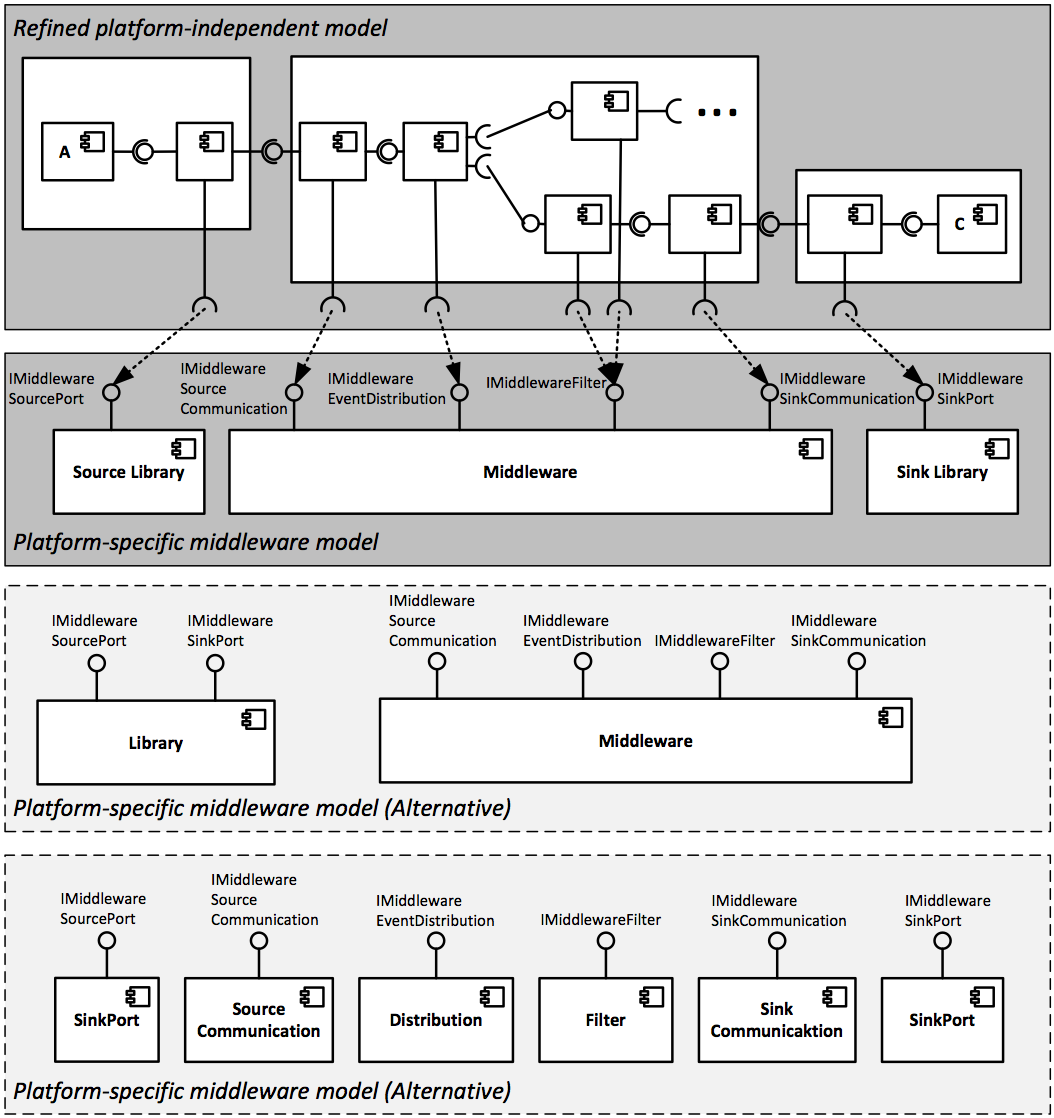
\includegraphics[width=1\textwidth]{images/grundlagen/middleware-model-weaving.png}
  \caption{Middleware-Schnittstellen}
  \label{img:weaving}
\end{figure}


\subsection{Performanzanalyse}
Die Palladio-Bench bietet eine Sammlung von Qualitätsanalysen mit Hauptfokus auf Performanz an. Daneben gibt es auch eine Zuverlässigkeits- und Kostenanalyse. Jedes Analysewerkzeug hat seine Vor- und Nachteile. Außerdem unterscheiden sie sich in ihrer Genauigkeit, Geschwindigkeit und ihrem Funktionsumfang. Im Palladio Kontext ist ein Analysewerkzeug eine Software, die eine Analysetechnik implementiert, die ein bestimmtes Analysemodell lösst. Mit lösen ist das Sammeln von Quallitätsmetriken aus dem Analysemodell gemeint. Diese Analysewerkzeuge können wie eine Blackbox verwendet werden, da ein Software-Architekt kein Spezialwissen benötigt um ein Analysewerkzeug zu verwenden. Nachdem ein Software-Architekt ein Modell erstellt hat, kann er ein Analysewerkzeug auswählen, das ihm Qualitätsmetriken vorhersagt. Mithilfe des Analysewerkzeugs \textbf{SimuCom} wurde im Rahmen der Masterarbeit die Performanz von MOMs vorhergesagt. SimuCom berechnet verschiedene Performanz Charakteristiken, darunter Antwortzeiten für Systeme und Komponenten. Außerdem wird die Auslastung der einzelnen Ressourcen berechnet. Für die Analyse transformiert SimuCom das Eingabemodell, mithilfe einer Modell-Zu-Text Transformation, in Java-Code. Der generierte Code wird im Anschluß an die Ausführungsumgebung von SimuCom angeschlossen und im nächsten Schritt ausgeführt. Nachdem die Simulation fertig ist, werden die Ergebnisse in der Palladio-Bench angezeigt. Dieser ganze Prozess ist vollautomatisch und benötigt keine Benutzerinteraktion. SimuCom wird im Rahmen der Masterarbeit bei der Modellierung und Evaluierung einer MOM verwendet.

\section{Benchmark}
Im Kontext der Informatik bezeichnet der Begriff Benchmark einen oder mehrere Tests, die ausgeführt werden, um die Leistungsfähigkeit von Computersystemen zu vergleichen. Hierfür wird zwischen verschiedenen Arten von Benchmarks unterschieden \cite{Lilja2004}. 
\begin{itemize}
\item \textbf{Mikrobenchmarks} sind Tests einzelner Komponenten ohne Interaktion mit dem Gesamtsystem. Sie werden meistens verwendet, um die maximal mögliche Leistungsfähigkeit einer Komponente zu testen.
\item \textbf{Synthetische Benchmarks} sind Tests künstlicher Instruktionsfolgen. Die getesteten Instruktionsfolgen können dabei in realen Anwendung vorkommen, müssen aber nicht.
\item \textbf{Anwendungsbenchmarks} beschreiben vollständige Programme, welche repräsentativ für eine bestimmte Klasse von Anwendungen sind. 
\end{itemize}
Im Rahmen der Masterarbeit wird ein Anwendungsbenchmark verwendet um eien MOM zu untersuchen und zu bewerten.

%- warum sind benchmark sinnvoll? bestehendes und einheitliches system mit dem man sich und andere vergleichen kann!!



